\chapter{Tätigkeitsbereiche und Aufgaben}
\label{sec:main}
\section{Überblick}
\label{sec:main:overview}
Ich habe im Rahmen meines Praktikums am Projekt \textit{SD4M - Smart Data for Mobility} mitgearbeitet.
Meine konkrete Aufgabe war die Aufbereitung und Integration verschiedener Daten und Datenbanken, damit diese im Projekt Verwendung finden können. Meine Hauptdatenquelle waren die Geodaten des OpenStreetMap\footnote{http://www.openstreetmap.org/} Projekts.
\subsection{Das Projekt SD4M}
\label{sec:main:overview:sd4m}
Das Projekt \textit{Smart Data for Mobilty}\footnote{http://sd4m.net/}, im folgenden \textit{SD4M} genannt, ist ein Verbundprojekt eines Konsortiums aus 5 Partnern und wird vom Bundesministerium für Wirtschaft und Energie gefördert.
Das Konsortium besteht aus 4 Wirtschaftsunternehmen und dem DFKI als Forschungseinrichtung.
\begin{compactitem}
  \item DB Systel GmbH (Konsortialführung)
  \item Deutsches Forschungszentrum für Künstliche Intelligenz GmbH
  \item idalab GmbH
  \item ]init[ AG für digitale Kommunikation
  \item PS-Team Deutschland GmbH & Co. KG
\end{compactitem}
Ziel des SD4M Projekts ist eine branchenübergreifende Serviceplattform, welche Daten der unterschiedlichen Mobilitätsanbieter (z.B. der Fahrplan der Deutschen Bahn) sowie öffentliche verfügbare strukturierte und unstrukturierte Daten (z.B. Twitter oder Facebook) miteinander verknüpft.
Diese verknüpften Daten sind für Endnutzer, aber auch für Unternehmen oder die öffentliche Verwaltung von Interesse.
In Abbildung \ref{fig:tweetXfahrplan} wird verdeutlicht, wie sich aus unstrukturierten Twitter-Daten Verspätungsinformationen für konkrete Verkehrsmittel extrahieren lassen.
Diese können dann Endnutzern oder den Mobilitätsanbietern zur Verfügung gestellt werden.
\begin{figure}
   \centering
   \fbox{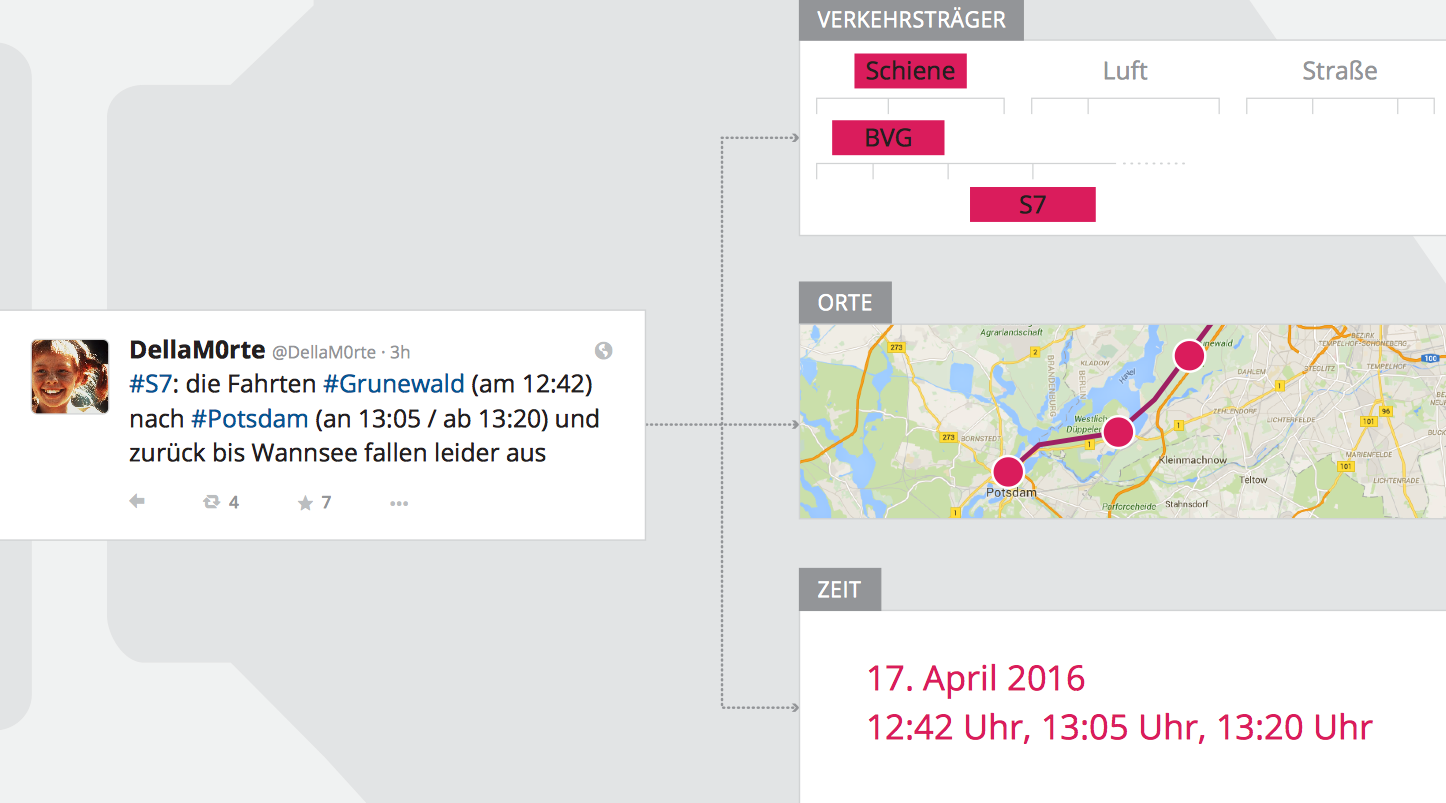
\includegraphics[width=1\textwidth]{gfx/sd4m_praesi_1.png}}
   \caption{Verknüpfung eines Tweets mit Fahrplandaten\protect\cite{WEB:SD4M:Presentation:2016}}
   \label{fig:tweetXfahrplan}
 \end{figure}

\section{Vorbereitung}
\label{sec:main:preparation}
Beim ersten Gespräch mit meinem Praktikumsbetreuer Dr. Philippe Thomas informierte ich mich, welche Programmierumgebungen und Programmiersprachen beim DFKI üblich sind.
Ebenfalls erkundigte ich mich nach einer vorhandenen OpenStreetMap Datenbank und weiterer vorhandener Infrastruktur.
Wir klärten, dass Java die geeignetste Sprache zur Lösung meiner Aufgaben war. 
Ebenfalls war eine OpenStreetMap Datenbank mit dem Datenbestand von Deutschland, sowie ein GitLab Repository Server vorhanden.
Da ich auf meinem eigenen Notebook entwickeln wollte, installierte ich mir einen virtuellen Linux-Server mit einer PostgreSQL Datenbank um einen kleinen Teil der OpenStreetMap Daten lokal auf meinem Rechner zu haben.
So konnte ich schneller entwickeln und mit einer wesentlich kleineren Datenbank testen.

\section{Aufgaben}
Meine Aufgaben während des Praktikums lassen sich in 3 Teilbereiche gliedern. Zunächst sollte ich eine Straßenliste aus OpenStreetMap extrahieren. Anschließend verknüpfte und aggregierte ich Daten, welche von der Deutschen Bahn geliefert wurden, mit Daten aus OpenStreetMap. In den letzten Wochen meiner Praxisphase gab es dann noch verschiedene Datenaufbereitungsaufgaben. Auf diese 3 Themengebiete werden in diesem Abschnitt nun eingegangen.

\subsection{Extraktion einer Straßenliste aus OpenStreetMap}

\subsubsection{Aufgabe}
Meine erste Aufgabe bestand darin, eine Liste aller Straßen Deutschlands inclusive dazugehöriger Geodaten zu erstellen.
Es sollte eine Java Anwendung erstellt werden, welche via Kommandozeilenargumenten konfiguriert wird, und die entsprechenden Ergebnisse in einer CSV-Datei ablegt.
Im Ergebnis sollten pro zusammenhängender Straße die Daten
\begin{compactitem}
  \item \textbf{ID}, eine fortlaufende Nummer
  \item \textbf{Name}, der Name der Straße
  \item \textbf{LineString}, der geographische Straßenverlauf im \textit{Well-Known-Binary (WKB)} Format (siehe Anlage \ref{sec:appendix:wkb})
  \item \textbf{GeoJSON}, der geographische Straßenverlauf im \textit{GeoJSON} Format (siehe Anlage \ref{sec:appendix:geojson})
\end{compactitem}
vorhanden sein.
Diese Daten sollen anschließend zur geographischen Verortung von Straßen aus Tweets genutzt werden.

\subsubsection{Lösung}
Für meinen Anwendungsfall, die Filterung und Extraktion von Daten, war es notwendig, die OpenStreetMap Daten in einer Datenbank vorliegen zu haben.
Die zwei populärsten Werkzeuge sind hierbei \textbf{osm2pgsql}\footnote{https://github.com/openstreetmap/osm2pgsql} und \textbf{Osmosis}\footnote{https://github.com/openstreetmap/osmosis}.
Der Hauptgrund hierfür ist dem Datenformat der OpenStreetMap Daten geschuldet. Wie im Anhang \ref{sec:appendix:osm:data} aufgezeigt, beinhalten die OpenStreetMap Daten \textit{Nodes} (Punkte mit Koordinaten) und \textit{Ways} (Linien aus Punkten). Die Importwerkzeuge haben die nützliche Eigenschaft, die Koordinaten aller Punkte eines Weges zu aggregieren.
Das ermöglicht die direkte Extraktion der Geometrie eines Ways ohne sich für jeden Way die Koordinaten aus den Daten selbst aggregieren zu müssen.
Beide Werkzeuge erzeugen unterschiedliche Datenbankschemata.
Das DFKI besitzt Datenbanken, in der die OpenStreetMap Daten Deutschlands mit osm2pgsql sowie Osmosis importiert wurden.
Ich informierte mich darüber, welches Schema am verlustfreisten ist.
\begin{quote}
``osm2pgsql is mainly written for rendering data with data. So it only imports tags which are going to be useful for rendering. ... whereas osmosis and osmium more geared towards truthfully representing a full OSM data set.''\footnote{http://giswiki.hsr.ch/Osm2pgsql}
\end{quote}
Ich entschied mich für die Datenbank im Osmosis-Schema, da diese den wahren Datenbestand am besten repräsentiert.\\
Eine physikalisch vorhandene Straße ist wird durch mehrere aneinanderhängende \textit{Ways} repräsentiert.
Wenn sich im Straßenverlauf ein Attribut (Ein \textit{Tag}) der Straße ändert, zum Beispiel ein hinzukommender Radweg, muss ein neues Teilstück diese neuen Gegebenheiten abbilden. Ein Beispiel hierfür findet sich in Anlage \ref{sec:appenix:osm:streets}.
 
\subsubsection{Schwierigkeiten}
Das Testen auf einer kleinen Datenbank beschleunigte zwar die Entwicklung, aber erst der erste Test auf der Hauptdatenbank zeigte massive Performanceprobleme auf.
Ich hatte wollte meine Anwendung möglichst speicherschonend gestalten und holte \\... meine Straßenobjekte einzeln aus der Datenbank...\\ Eine Messung zeigte jedoch dass die Datenbankabfrage der Flaschenhals \\... mit 300ms Abfragezeit und unter 1ms Verarbeitungszeit\\... also neugeschrieben und alles initial in den RAM zum verarbeiten...
\subsection{Verknüpfung von Daten der Deutschen Bahn mit Daten aus OpenStreetMap}
\subsubsection{Aufgabe}
\subsubsection{Lösung}
\subsubsection{Schwierigkeiten}
\subsection{Datenaufwertung??}
